\documentclass[12pt,letterpaper]{article}

\usepackage[titletoc]{appendix}
\usepackage[compatibility=false]{caption}

\usepackage{fullpage, listings, footnote, graphicx, multicol, enumitem, latexsym, placeins, csvsimple}
\usepackage{algorithm,algpseudocode}
\usepackage{subcaption, booktabs}

\usepackage[backend=biber,style=numeric]{biblatex}

\usepackage{hyperref}
\usepackage{cleveref}
\setdescription{leftmargin=\parindent,labelindent=\parindent}
\pdfpxdimen=\dimexpr 1 in/72\relax
\lstdefinestyle{appendixJava}{%
  belowcaptionskip=1\baselineskip,
  breaklines=true,
  xleftmargin=\parindent,
  xrightmargin=\parindent,
  language=Java,
  showstringspaces=false,
  basicstyle=\footnotesize,
  numberstyle=\tiny,
  keywordstyle=\bfseries,
  commentstyle=\itshape,
  numbers = left,
  tabsize=4,
}
\lstdefinestyle{appendixC}{%
  belowcaptionskip=1\baselineskip,
  breaklines=true,
  xleftmargin=\parindent,
  xrightmargin=\parindent,
  language=C,
  showstringspaces=false,
  basicstyle=\footnotesize,
  numberstyle=\tiny,
  keywordstyle=\bfseries,
  commentstyle=\itshape,
  numbers = left,
  tabsize=4,
}
\lstdefinestyle{appendixPy}{
  belowcaptionskip=1\baselineskip,
  breaklines=true,
  xleftmargin=\parindent,
  xrightmargin=\parindent,
  language=Python,
  showstringspaces=false,
  basicstyle=\footnotesize,
  numberstyle=\tiny,
  keywordstyle=\bfseries,
  commentstyle=\itshape,
  numbers = left,
  tabsize=4,
}
\lstdefinestyle{appendixXML}{
  belowcaptionskip=1\baselineskip,
  breaklines=true,
  xleftmargin=\parindent,
  xrightmargin=\parindent,
  language=XML,
  showstringspaces=false,
  basicstyle=\footnotesize,
  numberstyle=\tiny,
  keywordstyle=\bfseries,
  commentstyle=\itshape,
  numbers = left,
  tabsize=4,
}
\crefname{lstlisting}{listing}{listings}
\Crefname{lstlisting}{Listing}{Listings}
\author{Hawk Weisman\\CMPSC440: Operating Systems}
\title{Lab 7: Evaluating the Efficiency of File System Searching}
\date{Monday, April 7th, 2014}
\addbibresource{Lab7.bib}
\begin{document}
	\maketitle
	\tableofcontents
	\section {Introduction}

		\subsection{Comparison of Search Tools}
			\subsubsection{\texttt{grep}}

				Originally developed by Unix creator Ken Thompson, \texttt{grep} is a tool which searches text files for lines matching a regular expression. It was originally included in Research Unix Edition 4, released in 1973. It may be used to search single files, multiple files, directories, or the output of another program through input redirection. Like most early Unix tools, \texttt{grep} is implemented in C.

				\begin{figure}[H]
					\centering
					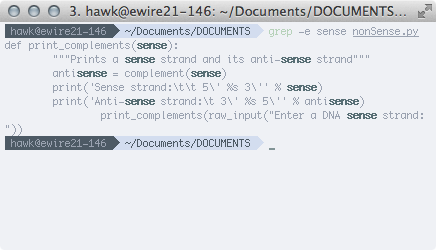
\includegraphics[resolution=72, scale = 0.75]{Figures/grep.png}
					\caption{A simple query and its results in \texttt{grep}.}
					\label{fig:grep}
				\end{figure}

			\subsubsection{\texttt{ack}}
				\texttt{ack} is a search tool based on \texttt{grep}, but optimized for the needs of programmers. \texttt{ack} is implemented entirely in Perl, and was written by Andy Lester. \texttt{ack} boasts several advantages over \texttt{grep}. 

				Unlike \texttt{grep}, which will only search entire directory trees if given the recursive (\texttt{-r}) argument, \texttt{ack} searches entire trees by default. Furthermore, \texttt{ack} defaults to searching only source code files, ignoring directories created by Subversion, Git, and other version control systems, backup files, and compiled binaries, making it significantly faster than \texttt{grep}\footnote{Do note that, while \texttt{grep} does not ignore these files by default, it can be instructed to. However, this process is fairly complex and time-consuming.} 

				Another feature of \texttt{ack} which programmers may find very useful is its' filetype specification system. This system allows programmers to use a single command-line flag, such as \texttt{--java}, to restrict the search to source code files from a given programming language. Specific languages can also be excluded from a search through the same system by prepending the word `no' to the flag, such as \texttt{--nojava}. This feature is available for most popular programming and markup languages.

				The \texttt{ack} documentation suggests that it is a superior replacement for \texttt{grep} in 99\% of use cases. However, it warns that \texttt{grep} may be faster when searching single files that are extremely large.

				\begin{figure}[H]
					\centering
					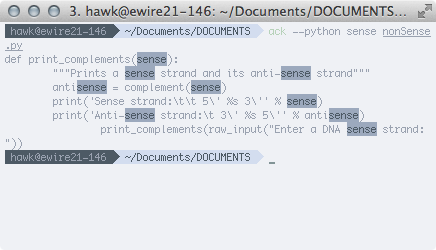
\includegraphics[resolution=72, scale = 0.75]{Figures/ack.png}
					\caption{A simple query and its results in \texttt{ack}.}
					\label{fig:ag}
				\end{figure}


			\subsubsection{The Silver Searcher}

				The Silver Searcher, also known by its' command-line name, \texttt{ag}\footnote{From the chemical abbreviation for silver.}, was developed by Geoff Greer and primarily intended as a replacement for \texttt{ack}. Greer claims that The Silver Searcher, which, like \texttt{grep}, is implemented in C, is three to five times faster than \texttt{ack}, leveraging both the speed advantage of \texttt{grep}'s compiled code, and the sophisticated ignore options of \texttt{ack}. The Silver Searcher also uses threads in order to take advantage of multiple CPU cores for additional speed. 

				The Silver Searcher can be used using a very similar syntax to \texttt{ack}, including the filetype specification flags, although this feature may only be used for restriction, and not for exclusion\footnote{For example, \texttt{ag} allows users to use the flag \texttt{--python} to restrict the search to Python source code files, but it does not allow \texttt{--nopython} to exclude Python source code files.}. This means that most graphical frontends or editor integration tools which are integrated with \texttt{ack} can be easily adapted to use \texttt{ag}.

				\begin{figure}[H]
					\centering
					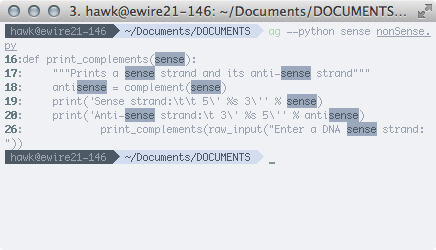
\includegraphics[resolution=72, scale = 0.75]{Figures/ag.png}
					\caption{A simple query and its results in \texttt{ag}.}
					\label{fig:ag}
				\end{figure}

			\subsubsection{Nautilus}

				Nautilus is a graphical filesystem browser

	\section{Methods}
		\subsection{Search Tool Setup and Configuration}

			The command-line search tools (\texttt{grep},  and \texttt{ag})  were tested on a MacBook Pro running OS X 10.9.2. While \texttt{grep} was installed by default, \texttt{ack} and \texttt{ag} were installed through Homebrew, the third-party package manager for Mac OS X, using the commands \texttt{brew install ack} and \texttt{brew install ag}, respectively. 



		\subsection{Search Tool Benchmarking}
			Tests were run using an IPython notebook, using the \texttt{subprocess} and \texttt{timeit} libraries. The \texttt{timeit} library provides a method, \texttt{timeit()}, which, when passed a string as an argument, runs the string as a Python statement and times its' execution. In this case, \texttt{timeit()} was passed calls to \texttt{subprocess.call()}, which in turn were given as an argument a string containing a command line to run the search tool being tested. Each query was run and timed 30 times, and an arithmatic mean and standard deviation for the times was calculated using the \texttt{numpy} library.

			The \texttt{subprocess.check\_output()} command was used to collect output for additional assessment. The output was searched using Python's regular expressions module, \texttt{re}, for patterns which match the search query, in order to count the number of instances of matches for the search pattern found. Additionally, unique file paths were counted in order to determine the number of files found by each search tool.

			The following search queries were run 30 times for each tool:
			\begin{description}
				\item[Query 1]{Search \url{~/Users/Documents} for Java source code files containing the word ``twitter''. The following command lines were used: \texttt{grep -r -i --include \textbackslash*.java twitter \textasciitilde/Documents} for \texttt{grep}, and \texttt{ag --java twitter \textasciitilde/Documents} for the Silver Searcher.}
				\item[Query 2]{Search \url{~/Documents} for Python source code files in which a class is defined. The command \texttt{grep -r -i --include \textbackslash*.py class \textasciitilde/Documents} was used for \texttt{grep}, and the command \texttt{ag --python class \textasciitilde/Documents} was used for \texttt{ag}.}
				\item[Query 3]{Search \url{~/Documents/DOCUMENTS/Projects/Knightingale} for Java source code files containing the word ``knightingale''. The command line \texttt{grep -r -i --include \textbackslash*.java knightingale \textasciitilde/Documents/DOCUMENTS/Projects/Knightingale} was used for \texttt{grep}, and \texttt{ag  --java knightingale \textasciitilde/Documents/DOCUMENTS/Projects/Knightingale} for \texttt{ag}.}
			\end{description}

	\section{Results and Analysis}
	\section{Discussion}
		\subsection{Difficulties and Challenges}
		\subsection{Further Research}
	\section{Advanced Use of Search Tools}

		Plugins exist for most popular text editors to integrate these search tools. For example, the \texttt{ag.vim} plugin allows Vim users to run \texttt{ag} searches from within that editor. Since my personal editor of choice is Sublime Text, I installed the SearchInProject plugin, which allows \texttt{grep}, \texttt{ack}, and \texttt{ag} searches to be run from within Sublime Text. This plugin is available at its' GitHub page, \url{https://github.com/leonid-shevtsov/SearchInProject_SublimeText}, or from the Package Control plugin manager for Sublime Text.
	\appendix
		\section{Experiment Source Code}
			\lstinputlisting[style=appendixPy, label={lst:notebook}]{CS440Lab7.py}
	\clearpage
	\addcontentsline{toc}{section}{References}
	\printbibliography

\end{document}